\section{Analysis strategy}
This analysis targets the $H^+$ production decaying into $tb$ in the single-lepton channel. The events that fulfil the selection described in Section~\ref{Hplustb:SectionEventSelection} are further divided into two types of disjoint analysis regions: signal regions and control regions. The control regions are used to improve the modelling of the \ttjets\ background, while several multi-variate techniques are used in the signal regions to improve the separation between signal and background events.

\subsection{Regions definition}

The analysis regions are categorised as a function of the number of reconstructed jets and $b$-tagged jets using the 70\% $b$-tagging operating point. A total of four signal regions are used, namely 5j3b, 5j$\geq$4b, $\geq$6j3b and $\geq$6j$\geq$4b. The nomenclature follows $X$j$Y$b, where $X$ denotes the number of jets and $Y$ the number of $b$-tagged jets.\\

Figure~\ref{Hplustb:cheeseplots} illustrates the background composition, which shows the large fraction of the \ttbar\ background, especially the \ttb\ component in the $\geq$4b regions. The 3b categories consist of a mixture of the three \ttbar\ components: 52\% of the 5j3b background are \ttl\ events, while 70\% of the $\geq$6j3b events is split equally between \ttb\ and \ttl\ events.\\

\begin{figure}[htbp]
    \RawFloats
    \begin{center}
    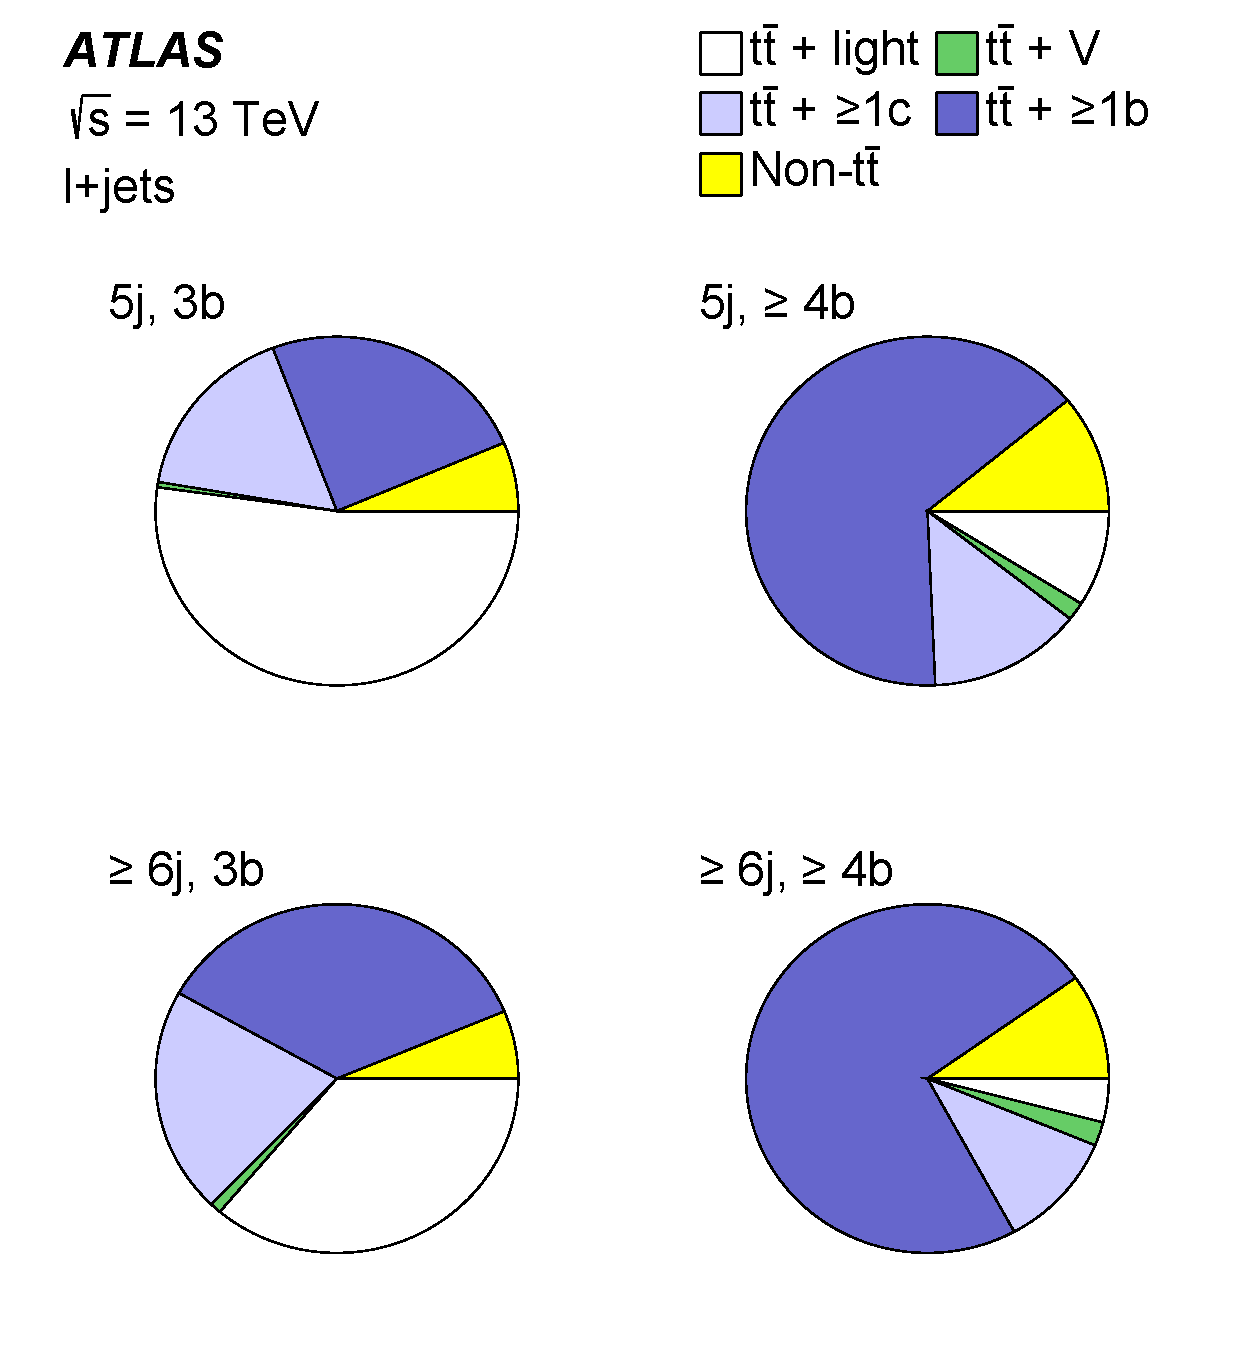
\includegraphics[width=0.75\textwidth]{HPLUSTB/cheeseplot.pdf}
    \caption{
        Background composition in the various analysis signal regions.
    }
    \label{Hplustb:cheeseplots}
    \end{center}
\end{figure}

Table~\ref{Hplustb:prefityields} shows the number of expected and selected events in the different regions, including the $\geq$5j2b selection which is used to derive weights to improve the \ttbar\ modelling, as described in the next section. The number of expected $H^+$ signal events for the 600 GeV mass hypothesis is also shown, whose contribution is less than 0.5\% in the $\geq$5j2b region and thus considered negligible. Another observation is that the region with the higher sensitivity in terms of $n_S/\sqrt{n_B}$ is the $\geq$6j$\geq$4b region.\\  %Table 6 shows the cut flow for each signal sample.

\begin{table}[htb]
    \scriptsize
    \addtolength{\leftskip} {-2cm} % menja marges
    \addtolength{\rightskip}{-2cm}
    \centering
    \begin{tabular}{l r r r r r}
        \toprule\toprule
          & $\geq$ 5j2b & {5j3b} & {5j$\geq$4b} & {$\geq$6j3b} & {$\geq$6j$\geq$4b}\\
          \midrule 
  $t\bar{t}$ + light        & 1365450 $\pm$ 420 & 44000 $\pm$ 8000  & 290 $\pm$ 130  & 31000 $\pm$ 6000  & 340 $\pm$ 180 \\ 
  $t\bar{t}$ + $\geq$1$b$   & 92380   $\pm$ 44 & 20500  $\pm$ 2400  & 2080 $\pm$ 240 & 30000 $\pm$ 4000  & 6100 $\pm$ 1500   \\ 
  $t\bar{t}$ + $\geq$1$c$   & 217830  $\pm$ 120 & 14000 $\pm$ 1600  & 440 $\pm$ 90   & 17800 $\pm$ 2400  & 910  $\pm$ 180   \\ 
  $t\bar{t}$ + $W$          & 3181    $\pm$ 5   & 109   $\pm$ 16    & 3.2 $\pm$ 0.6  & 230   $\pm$ 40    & 15.7   $\pm$ 2.8 \\ 
  $t\bar{t}$ + $Z$          & 3976    $\pm$ 12  & 300   $\pm$ 40    & 51  $\pm$ 7    & 650   $\pm$ 90    & 169  $\pm$ 24 \\ 
  $Wt$ channel              & 46190   $\pm$ 110 & 2300  $\pm$ 600   & 80  $\pm$ 50   & 1800  $\pm$ 800   & 150  $\pm$ 90 \\ 
  $t$ channel               & 19505   $\pm$ 74  & 790   $\pm$ 310   & 55  $\pm$ 21   & 600   $\pm$ 500   & 70   $\pm$ 50 \\ 
  Other top         & 1898    $\pm$ 8   & 125   $\pm$ 17    & 17.7  $\pm$ 3.3    & 190   $\pm$ 70    & 60   $\pm$ 24 \\ 
  $VV$ \& $V$ + jets        & 49830   $\pm$ 140 & 1700  $\pm$ 700   & 68  $\pm$ 25   & 1600  $\pm$ 600   & 120  $\pm$ 50 \\ 
  $t\bar{t}H$               & 2918    $\pm$ 2   & 530   $\pm$ 60    & 129 $\pm$ 20   & 1110  $\pm$ 130   & 420  $\pm$ 60 \\ 
\midrule      
  Total                     &1803170 $\pm$ 480 & 84000 $\pm$ 10000 & 3200$\pm$ 400 & 85000 $\pm$ 12000 & 8400 $\pm$ 1700 \\
\midrule
  Data                      &1830756           & 95852             & 4109          & 98929          & 10552 \\
\midrule  
\midrule\ $H^+\to tb$ 600 GeV             & 1911 $\pm$ 24   & 520 $\pm$ 40      & 73 $\pm$ 8    & 960 $\pm$ 80   & 279 $\pm$ 25  \\   
\bottomrule\bottomrule                               
    \end{tabular}
    \caption{Number of expected and selected events split according to the analysis regions. The $\geq$ 5j2b region is used to derive weights to improve the agreement between data and background. The quoted uncertainties include both statistical and systematic uncertainties except for the first column ($\geq$ 5j2b), which includes only statistical uncertainties. The predicted number of $H^+$ signal events for the 600 GeV mass hypothesis is also shown, assuming a cross-section times branching fraction of 0.32~pb.}
    \label{Hplustb:prefityields}
\end{table}

Figure~\ref{Hplustb:acceptance} shows the acceptance times efficiency of the $\geq$5j$\geq$3b inclusive selection per signal mass sample. It can be observed that the acceptance starts to decrease at the 1000~GeV $H^+$ mass, and this is due to the loss of jets and the characteristics of boosted regimes.

\begin{figure}[htbp]
    \RawFloats
    \begin{center}
    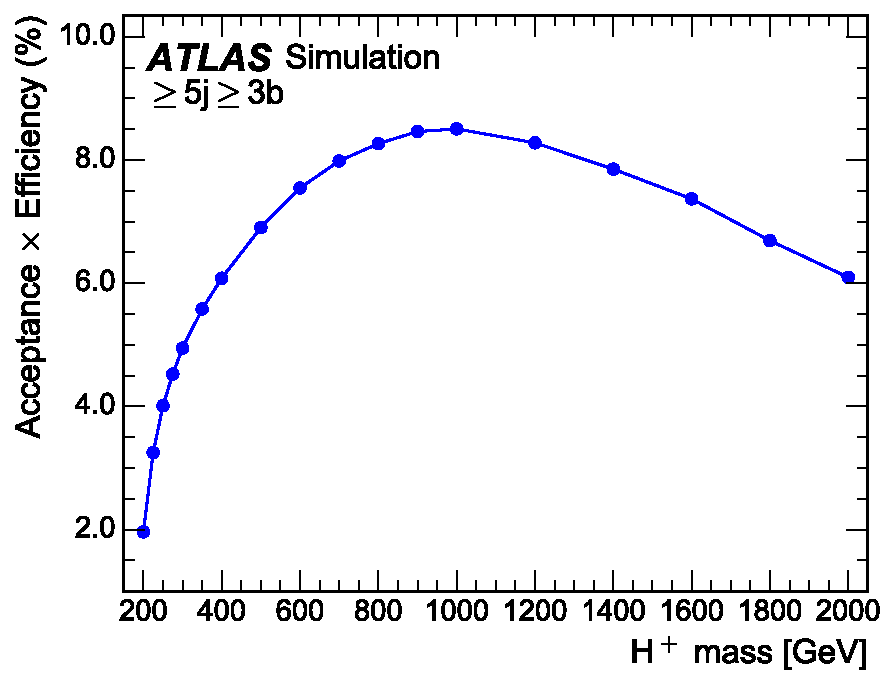
\includegraphics[width=0.75\textwidth]{HPLUSTB/acceptance.pdf}
    \caption{
        Total event acceptance of every $H^+$ signal sample in the analysis signal regions. Statistical uncertainties are included but hidden within the markers.
    }
    \label{Hplustb:acceptance}
    \end{center}
\end{figure}

\clearpage
\subsection{Reweighting technique}
\label{Hplustb:secRW}
The main background for this analysis is \ttjets, and its correct modelling is essential for an appropiate description of the data. It is observed that the simulation does not properly model high jet multiplicity events nor the hardness of additional jet emissions~\cite{ATL-PHYS-PUB-2018-009,10.1007/JHEP01(2021)033}.\\

To improve the data to MC agreement, data-based corrections are applied to the \ttbar\ samples. Since the mismodelling is assumed to be mainly due to the additional radiation in the parton shower, hence independent of the flavour of the associated jets, the corrections derived in the $\geq$5j2b regions are expected to improve the agreement in the 3b and $\geq$4b regions. The remaining discrepancies can be covered by the systematics model.\\

The corrections are derived for each jet multiplicity and as a function of \HTall, defined as the scalar \pT\ sum of jets and the lepton, i.e. all the selected objects. The reweighting factors for each jet multiplicity are expressed as:

\begin{equation}
    \label{Hplustb:RWeq}
    R(\HTall)=\frac{ \text{Data}(\HTall) - \text{MC}^{\text{non-\ttbar}}(\HTall) }{\text{MC}^{\text{\ttbar}}(\HTall)}
\end{equation}

and, by construction, assumes that any disagreement between data and MC comes from \ttbar. In this context, \ttbar\ includes the \ttb, \ttc\ and \ttl\ as well as single top $Wt$ contributions.\\

Figure~\ref{Hplustb:RWfactors} includes all the derived corrections, showing higher weights for large jet multiplicities. In general, the \HTall corrections have a hyperbolic behaviour (most visible in the 5j2b region) decreasing up to $\HTall > 800$ or 1000~GeV. Among various functions, the hyperbola plus a sigmoid functional form was found to best fit the weight distributions,

\begin{equation}
w=a+\frac{b}{(\HTall)^c} - \frac{d}{1+\exp(e-f\cdot\HTall)}.
\end{equation}

The eigenvalues of the fitted parameters' error matrix are used in the analysis fit model to include systematic uncertainties associated to the reweighting.\\

\begin{figure}[htb]
    \RawFloats
    \begin{center}
    \subfloat[$\ge$5j2b]{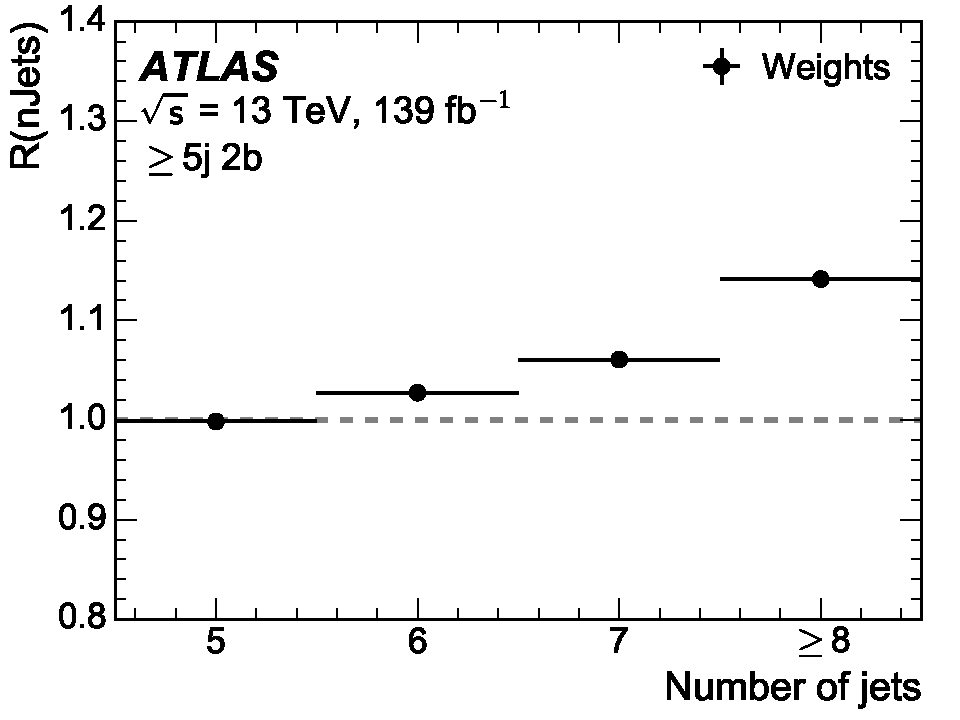
\includegraphics[width = 0.5\textwidth]{HPLUSTB/Reweighting/nominal_jets.pdf}} \\ 
    \subfloat[5j2b]{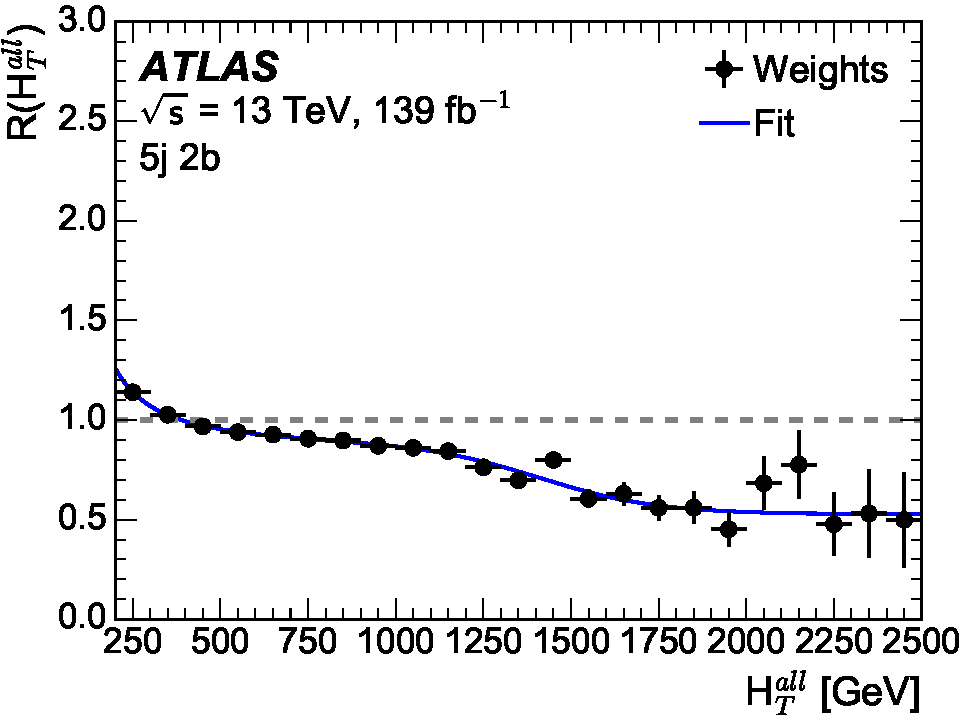
\includegraphics[width = 0.5\textwidth]{HPLUSTB/Reweighting/fitparsvar_hyp_5j.pdf}} 
    \subfloat[6j2b]{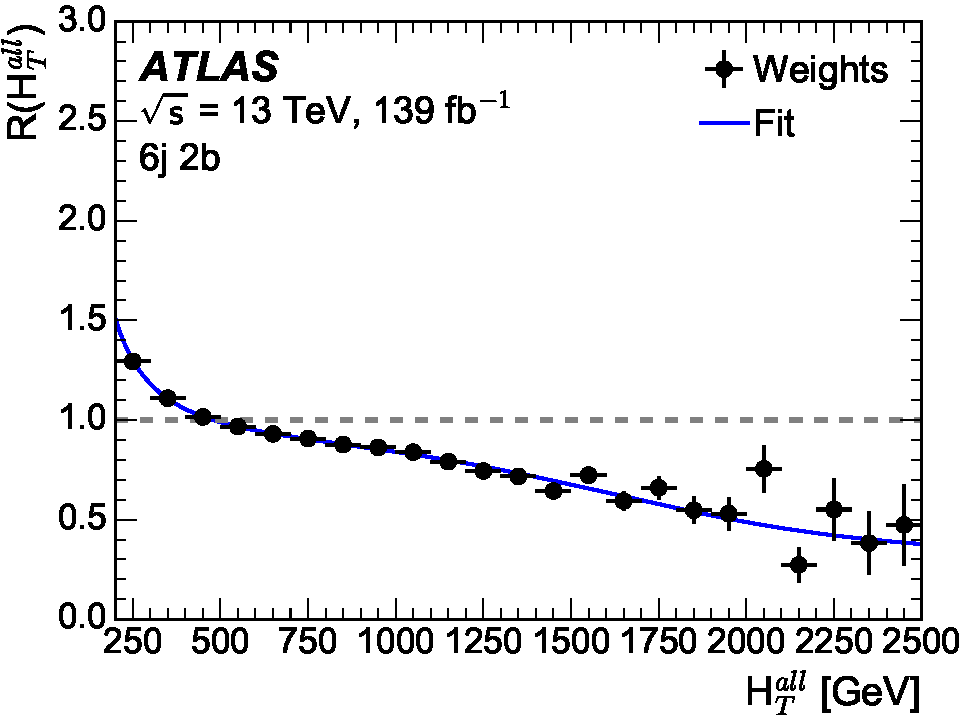
\includegraphics[width = 0.5\textwidth]{HPLUSTB/Reweighting/fitparsvar_hyp_6j.pdf}}  \\
    \subfloat[7j2b]{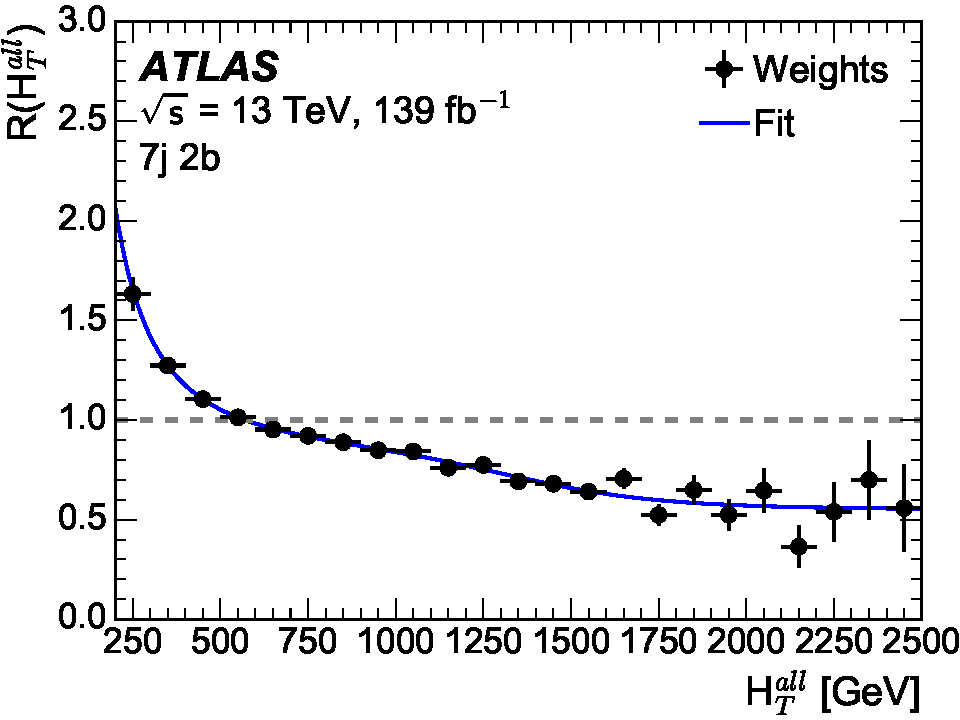
\includegraphics[width = 0.5\textwidth]{HPLUSTB/Reweighting/fitparsvar_hyp_7j.pdf}}
    \subfloat[$\ge$8j2b]{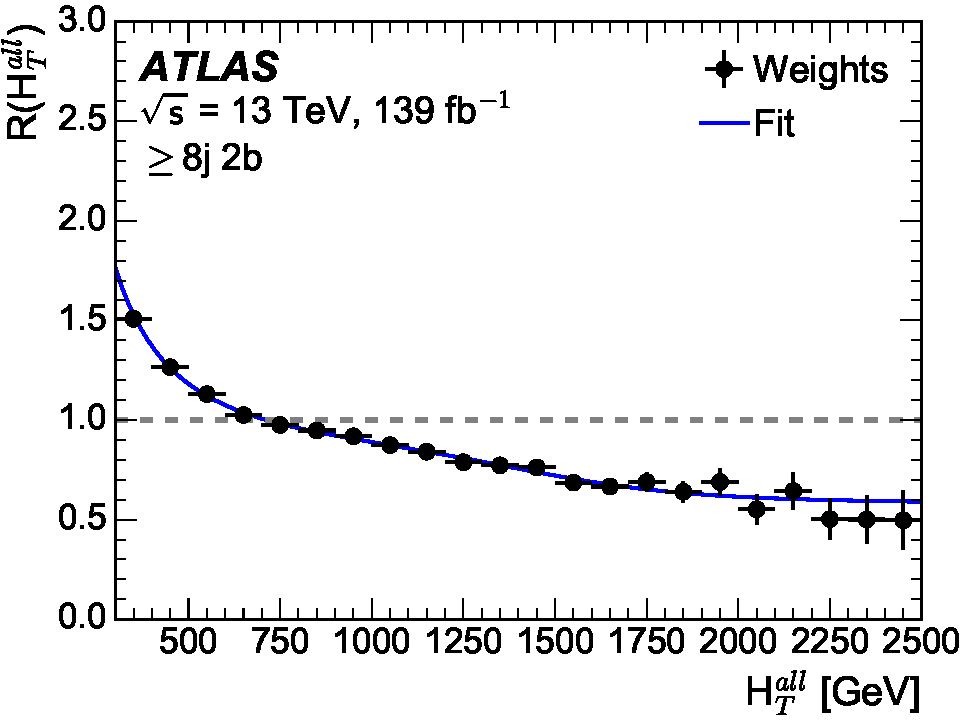
\includegraphics[width = 0.5\textwidth]{HPLUSTB/Reweighting/fitparsvar_hyp_8j.pdf}}
    \caption{Reweighting factors (weights) obtained from the comparison between data and simulation of the number of jets (a) and \HTall\ for various jet multiplicity selections (b) to (e).
    The errors in the data points include the statistical uncertainties in data and MC predictions.}
    \label{Hplustb:RWfactors}
\end{center}
\end{figure}

After applying these corrections, the agreement between simulation and data in the analysis regions improves, as can be seen in Figure~\ref{Hplustb:RWeffect}, which shows the leading jet \pT\ distributions before and after the reweighting. The shape of the distributions substantially improves and the remaining disagreement is mainly due to missing normalisations, which are obtained in the combined likelihood fit. All figures of this analysis in Section~\ref{chapter:Htbresults} are shown after the reweighting corrections are applied, unless stated otherwise.

\begin{figure}[htb]
    \RawFloats
    \begin{center}
    \subfloat[5j3b, unweighted]
    {\includegraphics[width = 0.33\textwidth]{HPLUSTB/Reweighting/unrw/plot_5jex3bex_jet_pt.pdf}}
    \subfloat[5j3b, reweighted] 
    {\includegraphics[width = 0.33\textwidth]{HPLUSTB/Reweighting/rw/plot_5jex3bex_jet_pt.pdf}} \\
     \subfloat[5j$\ge$4b, unweighted]
    {\includegraphics[width = 0.33\textwidth]{HPLUSTB/Reweighting/unrw/plot_5jex4bin_jet_pt.pdf}} 
     \subfloat[5j$\ge$4b, reweighted]
    {\includegraphics[width = 0.33\textwidth]{HPLUSTB/Reweighting/rw/plot_5jex4bin_jet_pt.pdf}}  \\
     \subfloat[$\ge$6j3b, unweighted] 
    {\includegraphics[width = 0.33\textwidth]{HPLUSTB/Reweighting/unrw/plot_6jin3bex_jet_pt.pdf}} 
     \subfloat[$\ge$6j3b, reweighted] 
    {\includegraphics[width = 0.33\textwidth]{HPLUSTB/Reweighting/rw/plot_6jin3bex_jet_pt.pdf}} \\ 
     \subfloat[$\ge$6j$\ge$4b, unweighted]
    {\includegraphics[width = 0.33\textwidth]{HPLUSTB/Reweighting/unrw/plot_6jin4bin_jet_pt.pdf}} 
     \subfloat[$\ge$6j$\ge$4b, reweighted]
    {\includegraphics[width = 0.33\textwidth]{HPLUSTB/Reweighting/rw/plot_6jin4bin_jet_pt.pdf}} \\  
    \caption{Comparison of the data and predicted leading jet \pT\ distributions before the fit in the four analysis signal regions before (left) and after (right) the reweighting is applied. The uncertainty bands include both statistical and systematic uncertainties, except for the cross-sections of the \ttb\ and \ttc\ backgrounds.
    The lower panels show the ratio of the data to the total prediction. 
    The hatched bands show the uncertainties before the fit to the data, which are dominated by systematic uncertainties. The $\chi^2$ per number of degrees of freedom ($\chi^2/\mathrm{ndf}$) and the $\chi^2$ probability are also shown. Statistical uncertainties on MC predictions and data are uncorrelated across bins, while systematic uncertainties on the predictions are correlated.}
    \label{Hplustb:RWeffect}
\end{center}
\end{figure}
\clearpage
\subsection{Multivariate techniques}

Multivariate techniques are used in this analysis to enhance the separation between signal and background. The kinematics of \ttb\ and signal events are very similar, and these techniques use different distributions as inputs to obtain a powerful discriminating variable.\\

The main classifier in this analysis is a parameterised NN trained over all signal and background, as described in Section~\ref{ML:SectionNN}. In the set of input variables, a kinematic discriminant is included to enhance the separation between a given $H^+$ sample and \ttjets.

\subsubsection{$\bm{H^+}$ parameterised NN}
\label{sec:HplusPNN}
The NN uses high-level variables as input, hence a simple and small architecture is enough to extract the discrimination power between signal and background. The architecture is sequential with two fully connected layers of 64 nodes and a single output node, implemented with the Python deep learning library, Keras~\cite{chollet2015keras}. The activation function used is the commonly employed \textsc{ReLU}, the loss function is the \textit{binary cross-entropy} and the optimiser is the Adam algorithm. Batch normalisation is performed to speed up the learning process. The dropout method is applied during the training at a 10\% rate. To further regularise the training, inputs are transformed to the same scale (same mean and variance) as the training set and a two-fold cross-validation setup is used. All signal samples are used in the training against all background samples, which are weighted according to their cross-sections.\\

Table~\ref{Hplustb:inputNNtable} shows the 15 variables used as input for the NN. The set includes several kinematic variables, geometric relations, event topology variables and jet multiplicities, which collectively provide a comprehensive characterisation of the events focusing on differences between the $H^+$ signal and the \ttbar\ background. In addition, the set includes a kinematic discriminant (a high-level variable described later in this section) and the $H^+$ mass. The NN is provided with the true $H^+$ mass, an input that distinguishes the different signals, which is a technique referred to as parameterised NN~\cite{Baldi_2016} and explained in Section~\ref{chapterML:PNN}. In signal events, the parameter is assigned to the corresponding $H^+$ mass used to generate them, while in background events a random value is assigned to each event, taken from the distribution of signal masses. This makes the NN to not directly use the parameter to perfectly classify the events, while the classification is optimised for each signal. As a result, the output of the NN is a function of the $H^+$ value. A total of four NNs are trained, one for each signal region: 5j3b, 5j$\geq$4b, $\geq$6j3b and $\geq$6j$\geq$4b.\\

\begin{table}[htb]
    \centering
    \small
    \begin{tabular}{l l}
        \toprule\toprule
        \multicolumn{1}{c}{Variable}  &  \multicolumn{1}{c}{Description}  \\
        \midrule
        $m_{H^+}$               & Parameter of the NN. $H^+$ mass hypothesis. \\
        $D$                     &   Kinematic discriminant of the $H^+$ mass hypothesis.   \\
        \HTjets &   Scalar sum of the transverse energy of all jets. \\
        Centrality         &   Centrality calculated using all jets and leptons.   \\
        $\pT^0$                 &   Leading jet \pT. \\
        $m^{\text{min}\Delta R}_{bb}$     &   Invariant mass of the closest $b$-jet pair. \\
        $\pT^4$  &   \pT of the fifth leading jet in \pT.  \\
        $H_1^{\mathrm{all}}$    &   Second Fox-Wolfram moment~\cite{foxwolframmoment} calculated using all jets and leptons.  \\ %https://journals.aps.org/prd/abstract/10.1103/PhysRevD.87.073014
        $\Delta R^{\text{avg}}_{bb}$ &   Average $\Delta R$ between all $b$-jet pairs in the event. \\
        $\text{min}\Delta R_{lep,bb}$  &   $\Delta R$ between the lepton and the pair of $b$-jets with smallest $\Delta R$.   \\
        $m^{\text{min}\Delta R}_{uu}$   &   Invariant mass of the untagged jet-pair with minimum $\Delta R$.\\
        $m^{\text{max}\pT}_{bb}$ &   Invariant mass of the $b$-jet pair with maximum \pT.  \\
        $m^{\text{max}m}_{bb}$  &   Maximal invariant mass of $b$-jets.   \\
        $m^{\text{max}\pT}_{jjj}$ &   Invariant mass of the jet triplet with maximum \pT.  \\
        $N_{\text{jets}}$ and $N_{b\text{-jets}}$ & jet and $b$-jet multiplicity. \\
        \bottomrule\bottomrule
        \end{tabular}
    \caption{List of variables included in the training of the NN.}
    \label{Hplustb:inputNNtable}
\end{table}

The kinematic discriminant, the \HTjets, the centrality and the leading jet \pT\ are consistently among the most important variables in the four trained regions. The NN output is obtained by evaluating the NN with the $H^+$ mass value set at the desired hypothesis. The NN distributions for signal and background in the analysis regions for the 200 and 800~GeV $H^+$ mass hypotheses are shown in Figure~\ref{Hplustb:NNshapes}. The shapes are significantly different between the two mass points, although the shape of the distributions transforms gradually from one mass to the next for two close-by masses. Let us notice that the shape of the background changes, since the same NN is evaluated but with a different $H^+$ mass value. The separation of the $H^+$ signal from the background is most difficult for low $H^+$ masses as the two processes have very similar kinematics and topology.

\begin{figure}[htb]
    \RawFloats
    \centering
    \subfloat[5j3b, $H^+$ 200 GeV]{\includegraphics[width = 0.5\textwidth]{HPLUSTB/NNshapes/INC_5j3b_200.pdf}}
    \subfloat[5j3b, $H^+$ 800 GeV]{\includegraphics[width = 0.5\textwidth]{HPLUSTB/NNshapes/INC_5j3b_800.pdf}}\\
    \subfloat[5j$\ge$4b, $H^+$ 200 GeV]{\includegraphics[width = 0.5\textwidth]{HPLUSTB/NNshapes/INC_5jge4b_200.pdf}}
    \subfloat[5j$\ge$4b, $H^+$ 800 GeV]{\includegraphics[width = 0.5\textwidth]{HPLUSTB/NNshapes/INC_5jge4b_800.pdf}} \\
    \subfloat[$\ge$6j3b, $H^+$ 200 GeV]{\includegraphics[width = 0.5\textwidth]{HPLUSTB/NNshapes/INC_ge6j3b_200.pdf}}
    \subfloat[$\ge$6j3b, $H^+$ 800 GeV]{\includegraphics[width = 0.5\textwidth]{HPLUSTB/NNshapes/INC_ge6j3b_800.pdf}} \\
    \subfloat[$\ge$6j$\ge$4b, $H^+$ 200 GeV]{\includegraphics[width = 0.5\textwidth]{HPLUSTB/NNshapes/INC_ge6jge4b_200.pdf}} 
    \subfloat[$\ge$6j$\ge$4b, $H^+$ 800 GeV]{\includegraphics[width = 0.5\textwidth]{HPLUSTB/NNshapes/INC_ge6jge4b_800.pdf}} \\

    \caption{Expected distributions of the NN output for $H^+$ masses of 200~GeV (left)
    and 800~GeV (right) for SM backgrounds and $H^+$ signal in the four signal regions.
    All distributions are normalised to unity.
    }
    \label{Hplustb:NNshapes}
\end{figure}
\clearpage
\subsubsection{Kinematic discriminant}
\label{Hplustb:SectionHplusDiscriminant}

The kinematic discriminant is a variable that accounts for the compatibility of an event to be signal or \ttbar\ background. This discriminant value is obtained by evaluating the probability density function~(pdf) of a given event under both the signal and background hypotheses. It can be defined in general as
\begin{equation}
    D(\textbf{x})=\frac{P^{\text{sig}}(\textbf{x})}{P^{\text{sig}}(\textbf{x})+P^{\text{bkg}}(\textbf{x})},
    \label{eq3:discriminant}
\end{equation}

where $P^{\text{sig}}(\textbf{x})$ and $P^{\text{bkg}}(\textbf{x})$ are the normalised pdf of the corresponding hypothesis, used below more generally as $P^{\text{hyp}}(\textbf{x})$. The value $D$ is computed for every signal mass and approaches to 1 if an event is identified as signal and to 0 if an event is identified as background.\\

The pdfs are based on kinematic information, from templates built from distributions using the four-momentum of the different objects of a given event. The jets are first matched to the final state partons identified at generator level. A quark is matched to a jet if $\Delta R$(jet,parton)$\leq 0.3$ and then, two categories are defined: when the full set of partons is successfully matched, the event is referred to as \textit{All Partons Matched}~(APM), while the event is called \textit{Missing Jet}~(MJ) if any of the partons fail to be matched. The MJ category consists mainly of events that are missing the matching of a quark produced by the $W$ boson, which are typically low in \pT\ and the associated jet is not reconstructed. Kinematic variables are built using up to the first six jets ordered in \pT. %talk about otherb? 
Concerning neutrinos, they are reconstructed solving the quadratic equation: $m_W^2 = (p_\ell + p_\nu)^2$, which assumes that all \MET\ is produced in the $W\to\ell\nu$ decay. In general, two solutions for the $z$ component of the neutrino momentum, $p_{z,\nu}$, are obtained and the solution with the lowest value. In the case that the equation does not return a real solution, the \MET\ is lowered until a solution is possible.\\

The discriminant is constructed by averaging the pdfs over all possible parton-jet combinations. By design, the individual pdf corresponding to the correct jet-parton combination contributes the most to the discriminant. This approach allows for the evaluation of the discriminant in real data events, as the true parton-jet associations are not required for the calculation. To reduce execution time, only up to the eight leading jets in \pT\ are used to compute kinematic variables. A flavour weight is assigned to each jet using the PCBT score in order to lower the contribution of the combination when a light jet is wrongly used as a $b$-parton or vice versa, thus reducing the impact of the incorrect combinations to the discriminant. The pdf of each hypothesis, signal and background, can be expressed as:
\begin{equation}
    P^{\text{hyp}}(\textbf{x})=\frac{\sum_{i=0}^N P^{\text{hyp}}_{b\text{tag}}(\textbf{x}_i)P^{\text{hyp}}_{\text{kin}}(\textbf{x}_i)}{\sum_{i=0}^N P^{\text{hyp}}_{b\text{tag}}(\textbf{x}_i)},
    \label{eq3:PDF}
\end{equation}
where $N$ is the total number of jet-parton combinations and $P^{\text{hyp}}_{\text{kin}}(\textbf{x})$ and $P^{\text{hyp}}_{\text{btag}}(\textbf{x}_i)$ are the kinematic pdf and the flavour weight for a given hypothesis, respectively. The kinematic variables and the $b$-tagging used to build the expressions for $P^{\text{hyp}}_{\text{kin}}$ and $P^{\text{hyp}}_{b\text{tag}}$ is described in detail below. The tagging weights can be expressed (for a single permutation) as

\begin{equation}
    P^{\text{hyp}}_{b\text{tag}}=P_b(j1)P_l(j2)P_l(j3)P_b(j4)P_b(j5)\begin{cases}1&5\text{j}\\P_l(j6)P_l(j7)P_l(j8)& \geq6\text{j},3b\\P_b(j6)P_l(j7)P_l(j8)&\geq6\text{j},\geq4b\end{cases}
\end{equation}

$P_b$ and $P_l$ are probabilities extracted from truth-matched events for a given jet matched to the corresponding hadron to be tagged as a $b$-jet or not, respectively. Each jet in the event is labelled from 1 to 8 for a single permutation. When an event contains more than 8 jets, all possible permutations involving 8 jets are taken into account. However, for events with more than 11 jets, only the first 8 jets in \pT\ are considered. This ensures a manageable number of permutations while still capturing the most relevant kinematic information from the jets in the event.\\

As the $H^+$ can decay either leptonically or hadronically, the kinematics involving the $H^+$ are a weighted combination of the two, according to the ratio of events in the two categories defined as $\omega_{lep}$ and $\omega_{had}$. Concerning neutrinos the same principle is applied only in the case of two neutrino solutions. To address the APM and MJ categories, $P^{\text{hyp}}_{\text{APM}}$ and $P^{\text{hyp}}_{\text{MJ}}$ are calculated individually following the previous definition (Equation~\ref{eq3:PDF}). Similarly, the final pdf in the discriminant is a weighted combination of the two, where the weight is the ratio between APM and MJ events.\\


\textit{Signal probability}

The signal kinematic probability $P^{\text{sig}}_{\text{kin}}$ is the product of the normalised kinematic probabilities extracted from the templates describing the phase space of the partonic final state. Templates are built for each signal mass sample by reconstructing the invariant masses for every truth-matched event for the signal, and are subdivided by region and by the categories already defined.\\

The template masses considered are the mass of the $H^+$, the mass of the hadronic $W$ ($M_{q\Bar{q}}$) and the masses of the leptonic and hadronic top-quarks ($m_{b_{lep}\ell\nu}$ and $m_{b_{had}q\Bar{q}}$). To minimise correlations between quantities, differences of invariant masses are used:

\begin{align}
    \begin{split} 
    \chi_{t_{had}}&=m_{b_{had}q\Bar{q}}-m_{q\Bar{q}} \\ 
    \chi_{H^+_{had}}&=m_{b_hb_{had}q\Bar{q}}-m_{b_{had}q\Bar{q}} \\
    \chi_{H^+_{lep}}&=m_{b_hb_{lep}\ell\nu}-m_{b_{lep}\ell\nu}\\
    \chi_{t_{had}b_4}&=m_{t_{had}b_4}-m_{t_{had}}=m_{b_{had}q\bar{q}b_4}-m_{b_{had}q\bar{q}}\\
    \chi_{t_{lep}b_4}&=m_{t_{lep}b_4}-m_{t_{lep}}=m_{b_{lep}\ell\nu b_4}-m_{b_{lep}\ell\nu}\\
    \end{split} 
\end{align}

where $b_h$ denotes the $b$-quark from the $H^+\to tb$ decay, $b_{had/lep}$ the one from the top quark $t_{had/lep}$ with the hadronically/leptonically decaying $W$ boson and $\chi_{t_{lep/had}b_4}$ refers to the recoil system of the $H^+$, from the $t$- and $b$-quarks generated in association with the boson. By introducing the two possible $H^+$ decays, the probability reads:

\begin{align}
    \begin{split}
        P^{\text{sig}}(\chi_{H^+})P^{\text{sig}}(\chi_{tb})=&\omega_{had}P^{\text{sig}}(\chi_{H^+_{had}})P^{\text{sig}}(\chi_{t_{lep}b_4})+\\
        &\omega_{lep}P^{\text{sig}}(\chi_{H^+_{lep}})P^{\text{sig}}(\chi_{t_{had}b_4}).
    \end{split}
\end{align}

The full kinematic signal probability for the different cases of jet multiplicities results
\begin{align}
    P_{\text{kin}}^{\text{sig}}&=P^{\text{sig}}(m_{W_h})P^{\text{sig}}(\chi_{t_{had}})P^{\text{sig}}(m_{t_{lep}})P^{\text{sig}}(\chi_{H^+})\begin{cases}1 & 5\text{j} \\ P^{\text{sig}}(\chi_{tj})&\geq6\text{j},3b\\P^{\text{sig}}(\chi_{tb})& \geq6\text{j},\geq4b\end{cases}.
\end{align}

It can be seen that the $H^+$ is used only in events with $\geq$6j regions as it cannot be built for 5j events. A light jet is assumed in $\geq$6j3b events. In the case of an event with two neutrino solutions, the leptonic quantities are computed using the two neutrinos and the probability is averaged with the fractions of $\omega_{1\nu}/\omega_{2\nu}$. These, analogous to $\omega_{had}/\omega_{lep}$, are the fraction of truth-matched events with two neutrino solutions that have the first or the second neutrino matched to the true neutrino.\\


\textit{Background probability}

The background kinematic pdf $P_{\text{kin}}^{\text{bkg}}$ follows a similar formula to the signal kinematic pdf. Almost all quantities can be reconstructed: the mass of the hadronic $W$ ($m_{q\bar{q}}$) and the mass of the leptonic and hadronic top-quark ($m_{b_{lep}\ell\nu}$ and $m_{b_{had}q\Bar{q}}$), for a total of three masses. Instead of the $H^+$ boson mass and its recoil system, the $m_{b\bar{b}}$ and the $\chi_{\ttbar}=m_{\ttbar}-m_{t_{had}}-m_{t_{lep}}$ systems are used.\\

In the 5j regions the $m_{b\bar{b}}$ system cannot be reconstructed, hence a pseudo-$H^+$ mass reconstructed with a light jet is used instead. Concerning the $\geq$6j3b region, two light-jets are used to build the $m_{j_hj_4}$, as the soft $b$-quark is typically tagged as a light jet and outputs a better performance than mixing jet flavours. Following this description, the background kinematic pdf is expressed as,
\begin{align}
    P_{\text{kin}}^{\text{bkg}}&=P^{\text{bkg}}(m_{W_h})P^{\text{bkg}}(\chi_{t_{had}})P^{\text{bkg}}(m_{t_{lep}})\begin{cases}P^{\text{bkg}}(\chi_{H^+}) & 5\text{j} \\ P^{\text{bkg}}(m_{jj})P^{\text{bkg}}(\chi_{t\bar{t}})&\geq6\text{j},3b\\P^{\text{bkg}}(m_{bb})P^{\text{bkg}}(\chi_{t\bar{t}})& \geq6\text{j},\geq4b\end{cases}.
\end{align}

The discriminant distributions for signal and background in the analysis regions for the 200 and 800~GeV $H^+$ masses are shown in Figure~\ref{Hplustb:Discriminantshapes}. Similar to the NN output, the shapes transform gradually from one mass to the next and the separation is most difficult for low $H^+$ masses.

\begin{figure}[htb]
    \RawFloats
    \centering
    \subfloat[5j3b, $H^+$ 200 GeV]{\includegraphics[width = 0.5\textwidth]{HPLUSTB/Discriminantshapes/INC_5j3b_200.pdf}} 
    \subfloat[5j3b, $H^+$ 800 GeV]{\includegraphics[width = 0.5\textwidth]{HPLUSTB/Discriminantshapes/INC_5j3b_800.pdf}}\\
    \subfloat[5j$\ge$4b, $H^+$ 200 GeV]{\includegraphics[width = 0.5\textwidth]{HPLUSTB/Discriminantshapes/INC_5jge4b_200.pdf}}
    \subfloat[5j$\ge$4b, $H^+$ 800 GeV]{\includegraphics[width = 0.5\textwidth]{HPLUSTB/Discriminantshapes/INC_5jge4b_800.pdf}}\\
    \subfloat[$\ge$6j3b, $H^+$ 200 GeV]{\includegraphics[width = 0.5\textwidth]{HPLUSTB/Discriminantshapes/INC_ge6j3b_200.pdf}}
    \subfloat[$\ge$6j3b, $H^+$ 800 GeV]{\includegraphics[width = 0.5\textwidth]{HPLUSTB/Discriminantshapes/INC_ge6j3b_800.pdf}}\\
    \subfloat[$\ge$6j$\ge$4b, $H^+$ 200 GeV]{\includegraphics[width = 0.5\textwidth]{HPLUSTB/Discriminantshapes/INC_ge6jge4b_200.pdf}}
    \subfloat[$\ge$6j$\ge$4b, $H^+$ 800 GeV]{\includegraphics[width = 0.5\textwidth]{HPLUSTB/Discriminantshapes/INC_ge6jge4b_800.pdf}}
    \caption{Expected distributions of the kinematic discriminant for $H^+$ masses of 200~GeV (left)
    and 800~GeV (right) for SM backgrounds and $H^+$ signal in the four signal regions.
    All distributions are normalised to unity.
    }
    \label{Hplustb:Discriminantshapes}
\end{figure}
\clearpage